\documentclass{article}


% if you need to pass options to natbib, use, e.g.:
%     \PassOptionsToPackage{numbers, compress}{natbib}
% before loading neurips_2022


% ready for submission
\usepackage[preprint,nonatbib]{neurips_2022}


% to compile a preprint version, e.g., for submission to arXiv, add add the
% [preprint] option:
%     \usepackage[preprint]{neurips_2022}


% to compile a camera-ready version, add the [final] option, e.g.:
%     \usepackage[final]{neurips_2022}


% to avoid loading the natbib package, add option nonatbib:
% \usepackage[nonatbib]{neurips_2022}


\usepackage[utf8]{inputenc} % allow utf-8 input
\usepackage[T1]{fontenc}    % use 8-bit T1 fonts
\usepackage{hyperref}       % hyperlinks
\usepackage{url}            % simple URL typesetting
\usepackage{booktabs}       % professional-quality tables
\usepackage{amsfonts}       % blackboard math symbols
\usepackage{nicefrac}       % compact symbols for 1/2, etc.
\usepackage{microtype}      % microtypography
\usepackage{xcolor}         % colors
\usepackage{graphicx}
\usepackage{subcaption}
\usepackage{amsthm,amsmath,amssymb}
\usepackage[noabbrev,capitalise]{cleveref}

\theoremstyle{definition}
\newtheorem{definition}{Definition}[section]

\newcommand{\ZZ}{\mathbb{Z}}
\newcommand{\braket}[1]{\langle #1 \rangle}
\newcommand{\Braket}[1]{\left\langle #1 \right\rangle}
\newcommand{\norm}[1]{| #1 |}


\title{Final Project: Grokking Phenomenon Reproduction}


% The \author macro works with any number of authors. There are two commands
% used to separate the names and addresses of multiple authors: \And and \AND.
%
% Using \And between authors leaves it to LaTeX to determine where to break the
% lines. Using \AND forces a line break at that point. So, if LaTeX puts 3 of 4
% authors names on the first line, and the last on the second line, try using
% \AND instead of \And before the third author name.


\author{%
  Kecen Sha \thanks{Equal contribution.} \\
  2200010611\\
  \And
  Yuziheng Wu \footnotemark[1]\\
  2200010878 \\
  \And
  Di Yue \footnotemark[1]\\
  2100012961 \\
  % \And
  % Coauthor \\
  % Affiliation \\
  % Address \\
  % \texttt{email} \\
  % \And
  % Coauthor \\
  % Affiliation \\
  % Address \\
  % \texttt{email} \\
}


\begin{document}


\maketitle

\begin{abstract}
    % Grokking, a phenomenon that the generalization of a neural network happens much later than the convergence of its training loss, has received increasing attention from both learning theory and application since it was first introduced by [Power et al., 2022].
    We reproduce the grokking phenomenon [Power et al., 2022], that a neural network generalizes long after it memorizes the training data, for modular addition problem, and provide an explanation based on [Kumar et al., ICLR 2024].
    \footnote{All the code and supplementary materials are available at: \url{https://github.com/tnediserp/MIML-grokking}}
\end{abstract}

\section{Introduction}
\label{sec:intro}

In the study of machine learning, it is an important goal to understand the generalization dynamics of neural networks.
Typically, the model's generalization ability can be well reflected by its performance on the training data.
However, when training neural networks for certain problems, generalization may occur long after the model overfits the training data. 
This striking phenomenon is called \emph{grokking}~\cite{Grokking}. 
Ever since it was first introduced, exhausted efforts have been made to understand grokking from a theoretical viewpoint.
For example, grokking is explained by the hardness of representation learning~\cite{LiuKNMTW22},
the effect of weight decay and weight norm decrease~\cite{Grokking_circuit_efficiency,LiuMT23}
and the transition between different training regimes~\cite{KumarBGP24,MohamadiLWS24}.

Among all the learning tasks where grokking can be observed, the most well-studied one might be the \emph{modular addition problem}~\cite{Grokking,KumarBGP24,MohamadiLWS24,Gromov}.
Specifically, given a fixed prime number $p$, consider learning the output of the modular arithmetic: % where each equation consists of $K$ summands and is represented as a string:
\begin{equation}
    a_{1} + a_{2} + \cdots + a_{K} = b,
    \label{eqn:modular_addition}
\end{equation}
where both the individual summands $a_i$ and the sum $b$ are elements of the finite field $\mathbb{Z}/p\mathbb{Z}$.
We model \eqref{eqn:modular_addition} as a classification problem, where classes are labeled by integers $b \in \{0, 1, \dots, p-1\}$.
We mainly focus on the case $K=2$, and discuss general $K$-wise addition in \cref{sec:subtask4}.

% Our experiments are divided into 4 parts in section 3. \ref{sec:subtask1} reproduces the grokking phenomenon stated in \cite{Grokking} and study the effect of $\alpha$ on grokking phenomenon. \ref{sec:subtask2} uses other models such as LSTM and MLP to conduct the same task. \ref{sec:subtask3} investigates the impact of different optimizers(with different hyper-Parameters such as learning rate, weight decay and dropout) to grokking phenomenon. \ref{sec:subtask4} explores the grokking phenomenon for different $K$.  

% At the end of our report we give some explanations on grokking phenomenon, mainly based on \cite{JacotHG18}.


\section{Notations and Problem Setup}
\label{sec:prelim}

Throughout, we let $p$ be a prime and denote $\ZZ_p = \{0, 1, \dots, p-1\}$ to be the additive group modulo $p$.
Each of the arithmetic equations in $\ZZ_p$ is initially represented by a token string \texttt{[`a', `+', `b', `=', `c']}.
Let $d_{\mathrm{tok}}$ be the total number of tokens.
For each token $t$, denote $e_t \in \RR^\dtok$ to be the one-hot encoding of $t$, (i.e., $e_t$ has only the $t$-th coordinate being $1$).
For $a \in \ZZ_p$, we sometimes denote its corresponding token also by $a$, without causing any confusion.

Our whole dataset includes all $p^K$ (tokenized) equations in $\ZZ_p$.
Given the training data fraction $\alpha\in(0,1)$, we randomly take an $\alpha$-fraction of the dataset as the training set and the rest as the validation set.

Our classification model $f$ takes as input $(e_{a_1}, e_{a_2}, \dots, e_{a_K}) \in \RR^{K \cdot \dtok}$, where $a_i \in \ZZ_p$, and outputs a prediction vector $\mathbf{y} \in \RR^{\dtok}$.
Throughout the model is evaluated by cross-entropy loss with the target output $e_{a_1 + a_2 + \dots + a_K}$.
% Specifically, we denote the target function to be $f^*(e_{a_1}, e_{a_2}, \dots, e_{a_K}) = e_{a_1 + a_2 + \dots + a_K}$.



% is such an equation string. Each character within the string, including digits and the addition operator, is transformed into a one-hot vector representation. This encoding scheme assigns a unique binary vector to every possible character.

% The output of the model is also designed as a one-hot vector, corresponding to the predicted value of $b$ after decoding. During the training phase, the target output is the actual sum $b$, computed as the sum of $K$ modular numbers modulo $p$. The objective of the training process is to adjust the model parameters so that it learns to accurately predict the correct modular sum $b$ given any valid input equation string.

% We mainly focus on the phenomenon when $K=2$. In this case, we first generate all $p^2$ equations and shuffle them randomly. Given the training data fraction $\alpha\in(0,1)$, we take the first $\alpha$ data as training set and the rest as validation set.

\section{Experiments}
\subsection{Reproducing the Grokking Curve}
\label{sec:subtask1}
\subsection{Grokking Phenomenon of Other Models}
\label{sec:subtask2}
\subsection{Effects of Different Hyperparameters}
\label{sec:subtask3}

In this task, we study the effects of hyperparameters such as the optimizer, learning rate, weight decay, dropout and batch size.
For all experiments in this section, we set $p = 97$ and use the transformer model.
Our baseline setting has the same hyperparameters as mentioned at the beginning of \cref{sec:subtask1}.
% The results are shown in \cref{fig:different_settings}.
% Similarly, the training accuracies raise up to $99\%$ within $10^3$ steps in most experiments, but the validation accuracies differ from each other.

\begin{figure}[!ht]
    \centering
    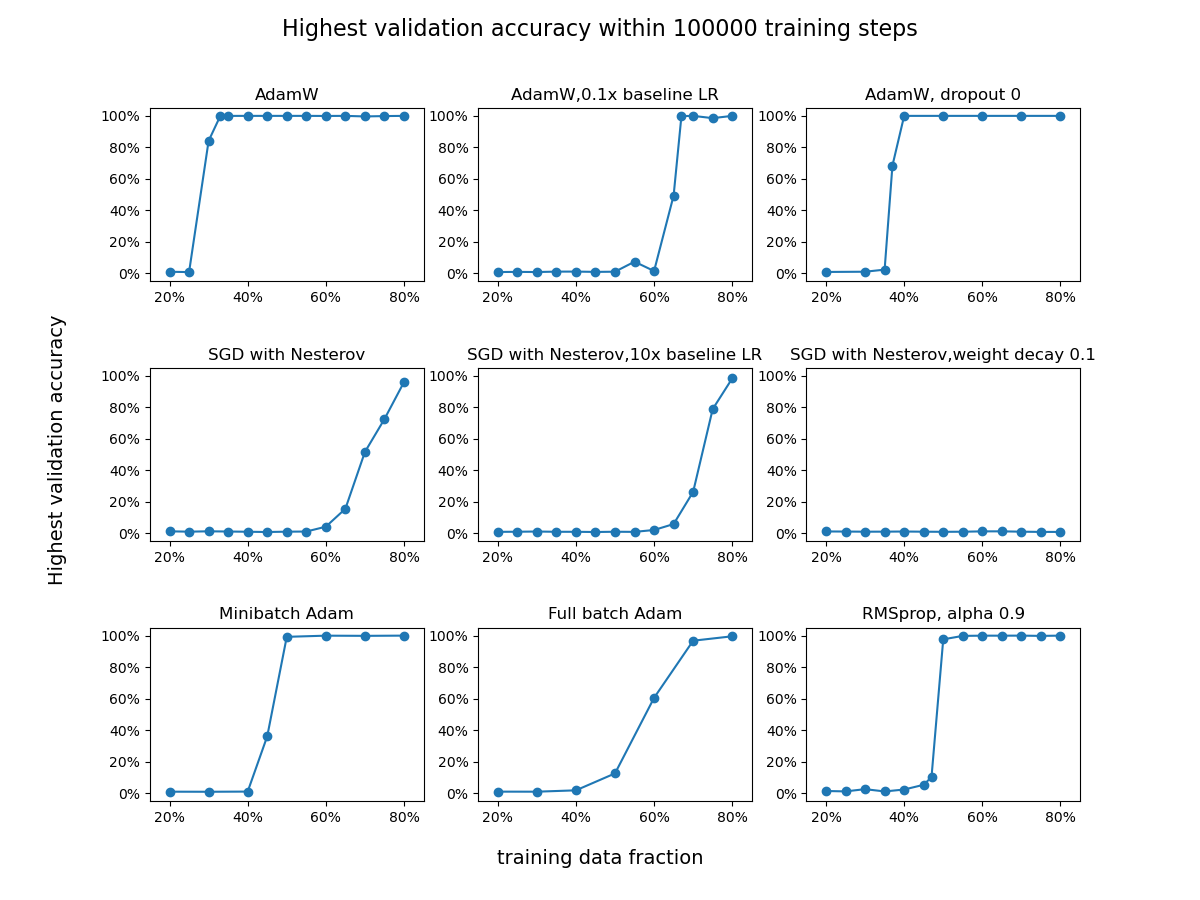
\includegraphics[width=0.9\textwidth]{fig/different_settings/different_settings.png}
    \caption{Grokking phenomenon for different settings.
    Top left: Baseline setting (see \cref{sec:subtask1}).
    Top center: Baseline setting with learning rate $10^{-4}$.
    Top right: Baseline setting with dropout $0$.
    Middle left: SGD with Nesterov, weight decay $0$, learning rate $10^{-3}$.
    Center: SGD with Nesterov, weight decay $0$, learning rate $10^{-2}$.
    Middle right: SGD with Nesterov, weight decay $0.1$, learning rate $10^{-3}$.
    Bottom left: Mini batch Adam with weight decay $0$.
    Bottom center: Full batch Adam with weight decay $0$.
    Bottom right: RMSprop with $\alpha = 0.9$, weight decay $0$.
    }
    \label{fig:different_settings}
\end{figure}
\begin{figure}[!ht]
    \centering
    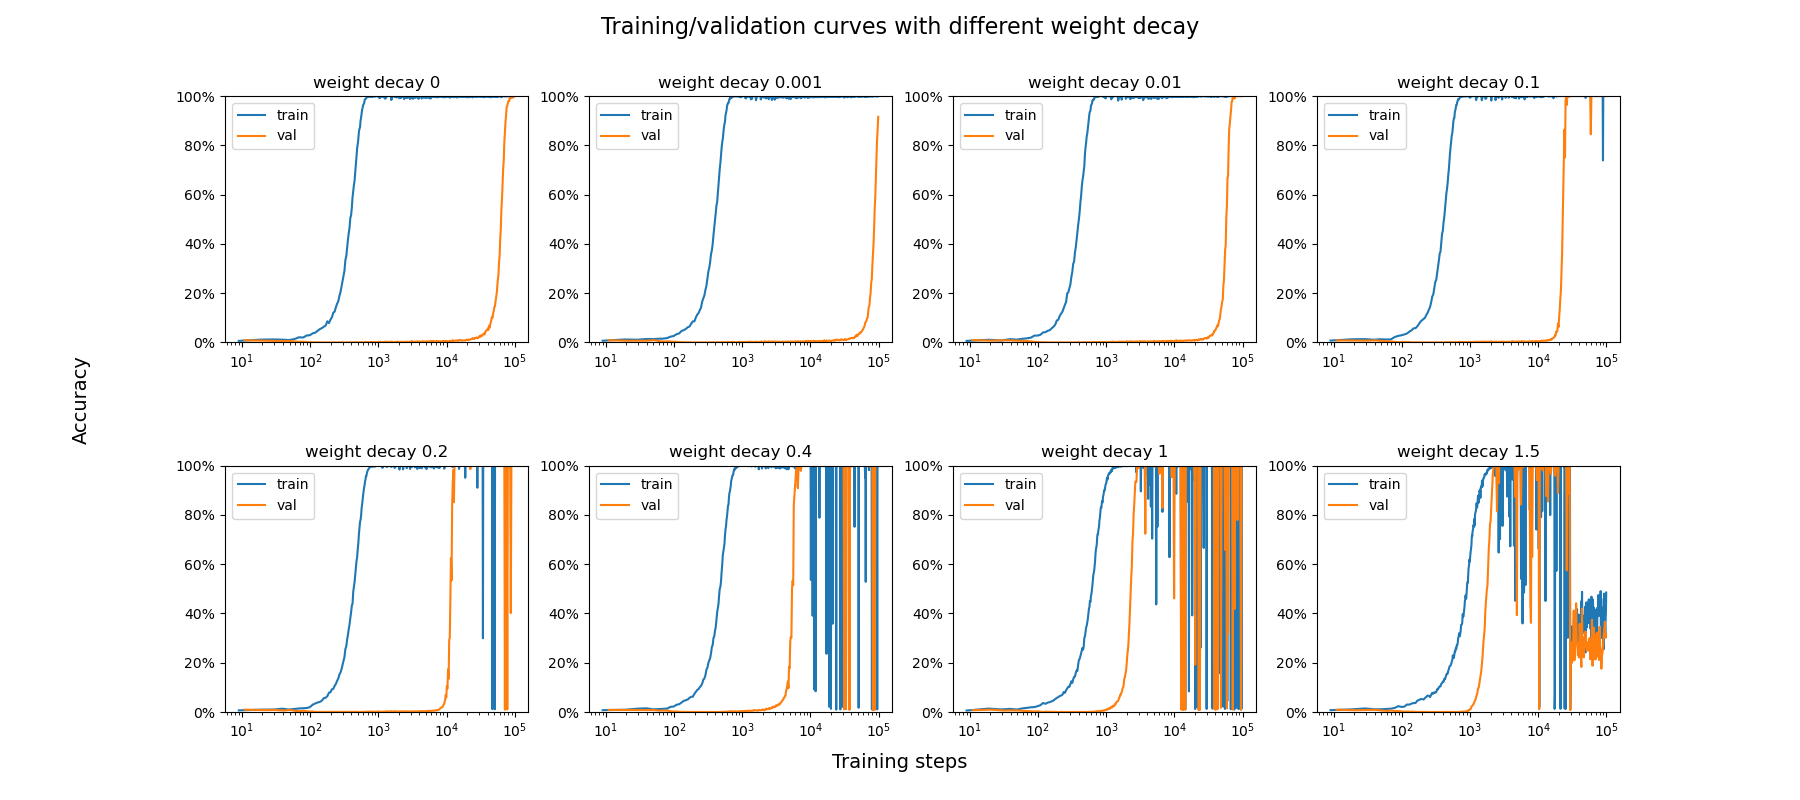
\includegraphics[width=0.9\textwidth]{fig/weight_decay/weight_decay.png}
    \caption{Grokking phenomenon for different weight decay}
    \label{fig:different weight_decay}
\end{figure}

It can be seen from \cref{fig:different_settings} that the model generalizes well in the baseline setting for training data fraction $\alpha = 33\%$, but does not generalize even for $\alpha = 60\%$ when the learning rate is changed into $10^{-4}$.
This is because a small learning rate slows down training.
However, big learning rates do not necessarily speed up training, which can be seen by comparing the first two figures on the second row. 
Removing dropout has little impact on AdamW (top right).
Adding weight decay makes SGD's training even worse (middle right).
As for the comparison between optimizers, under the same learning rate and dropout settings, AdamW is the best and SGD with Nesterov acceleration is the worst.
RMSprop and mini batch Adam have acceptable performance when $\alpha \geq 50\%$, while full batch Adam needs to exceed $70\%$ to reach the same level.

We further study the impact of weight decay by training the transformer model with AdamW optimizer with different weight decay.
The results are plotted in \cref{fig:different weight_decay}.
As the weight decay increases, the generalization becomes easier, and the grokking phenomenon becomes less obvious. 
However, it is worth noting that when the weight decay exceeds $0.2$, there are occasional ``rollback'' phenomena in training accuracy and validation accuracy on certain training steps, which occur more frequently as the weight decay increases. 
When the weight decay is $1.5$ and the number of training steps exceeds $3 \times 10^4$, accuracy cannot even be restored. 
The reason is worth further exploration, but at least it tells us that the selection of training steps does not need to be too large.
\subsection{Grokking for $K$-Wise Modular Addition}
\label{sec:subtask4}

\section{An Explanation of the Grokking Phenomenon}
\label{sec:explanation}

In this section, we provide an explanation of the grokking phenomenon based on~\cite{KumarBGP24}, which claims that grokking happens as a transition between different regimes of training.
We first briefly review the kernel regime and rich regime defined in~\cite{KumarBGP24} in \cref{subsec:regimes}, and illustrate how they help explain the grokking phenomenon for modular addition in \cref{subsec:explain_by_regimes}.

\subsection{Kernel Regime And Rich Regime}
\label{subsec:regimes}

We have the following definition of neural tangent kernel (NTK).

\begin{definition}[Neural Tangent Kernel~\cite{JacotHG18,KumarBGP24}]
    \label{def:NTK}
    Let $\Theta$ be the parameter space and $\mathcal{X}$ be the input space.
    Let $f \colon \Theta \times \mathcal{X} \to \mathcal{Y}$ be a neural network.
    For $\theta \in \Theta$, the \emph{neural tangent kernel} of $f(\theta, \cdot)$ is defined as 
    \begin{align*}
        K_\theta(\mathbf{x}, \mathbf{x}') := \nabla_\theta f(\theta, \mathbf{x}) \nabla_\theta f(\theta, \mathbf{x}')^\top, 
        \quad \forall \mathbf{x}, \mathbf{x}' \in \mathcal{X}.
    \end{align*}
\end{definition}

In the \emph{kernel regime}, we have the following approximation of the model output, 
\begin{align}
    f(\theta, \mathbf{x}) \approx f(\theta_0, \mathbf{x}) + \Braket{\nabla_{\theta} f(\theta_0, \mathbf{x}), \theta - \theta_0}.
    \label{eqn:tayler}
\end{align}
Note that the right-hand side of \eqref{eqn:tayler} is linear in $\theta$, which means that $f(\theta, \cdot)$ has approximately the same expressivity as the kernel method with respect to $K_{\theta_0}$, as defined in \cref{def:NTK}.
Under gradient descent, the model's parameters $\theta$ are restricted to the affine subspace $W := \mathrm{span}\{\nabla_{\theta} f(\theta_0, \mathbf{x}_i)\}_{i=1}^n$.
Therefore, the model will first converge to the local optimal solution $\theta_W^* \in W$ in the kernel regime.
\emph{This corresponds to the stage where the model overfits the training data but does not generalize.}

When the model begins to learn important non-linear features, it will escape $W$ and enter the \emph{rich regime}, where it finally converges towards the global optimal solution $\theta^*$.
\emph{This corresponds to the generalization phase in the grokking phenomenon.}

It is worth mentioning that normalization methods such as weight decay accelerates generalization by encouraging the model to escape from the kernel regime, which is consistent with our experiment results in \cref{sec:subtask3} (see \cref{fig:different weight_decay}).


\subsection{Regime Transition in Modular Addition Problem}
\label{subsec:explain_by_regimes}

We further illustrate how grokking is related to the transition between the two aforementioned regimes in the modular addition problem.
We first rewrite the target function $f^*$ as 
\begin{align*}
    f^*(e_a, e_b) = e_{a+b} = H^a e_b = H^b e_a, 
\end{align*}
where $H = \sum_{j=0}^{p-1} e_{j+1} e_{j}^\top$ is the $p \times p$ cyclic permutation matrix.
When the first (second) coordinate of $f^*$ is fixed, it becomes a simple linear function of the second (first) coordinate.
Following this observation, we consider the following generalized version of $f^*$.

Let $A$ be any non-empty subset of $\ZZ_p$, and $E(A) := \{e_a \colon a \in A\}$. Denote $E(\ZZ_p) := \{e_0, e_1, \dots, e_{p-1}\}$.
Define $f_A^* \colon E(A) \times E(\ZZ_p) \to E(\ZZ_p)$ to be the restriction of $f^*$ on $E(A) \times E(\ZZ_p)$.
Intuitively, the smaller $\norm{A}$ is, the closer $f_A^*$ is to a linear map.
We define $\lambda := \frac{\norm{A}}{p} \in (0, 1]$ to be a measure of the ``non-linearity'' of $f_A^*$.
Specifically, $f^* = f_{\ZZ_p}^*$, and thus has non-linearity $1$.

To prove the explanations in \cref{subsec:regimes}, we study how the non-linearity $\lambda$ influences the grokking phenomenon.
For each given $\lambda$, we sample a random subset $A \subseteq \ZZ_p$ of size $\lambda p$.
We then train a $2$-layer MLP on $A \times \ZZ_p$ with training data fraction $\alpha = 0.6$, SGD optimizer and weight decay $0$ to learn the target function $f_A^*$.
The results are shown in \cref{fig:acc_and_loss_different_lambda}.

\begin{figure}[!ht]
    \centering
    \begin{subfigure}{0.45\textwidth}
        \centering
        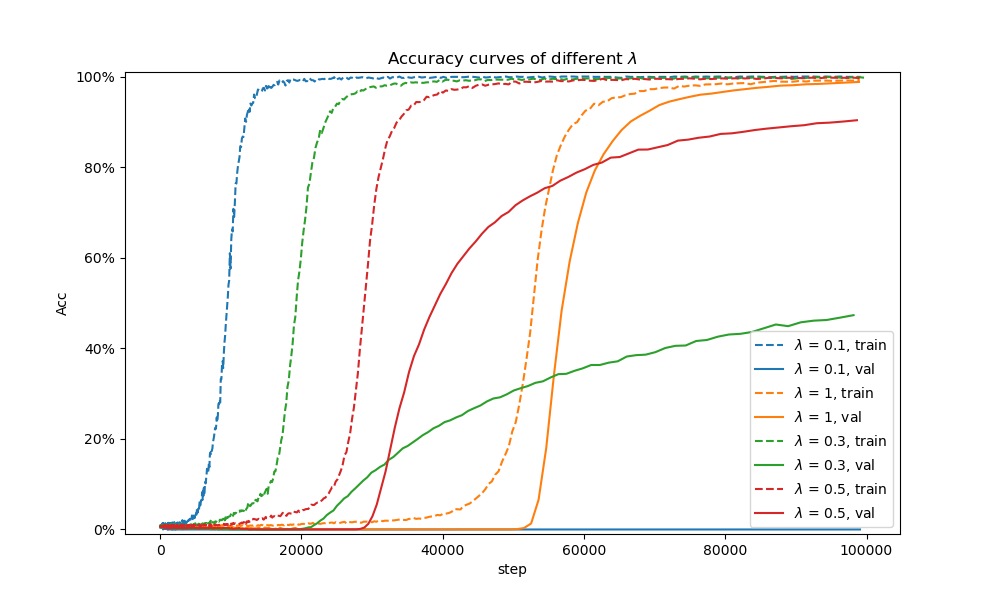
\includegraphics[width=\linewidth]{fig/grokking_curves/different_Afraction_acc.png}
        \caption{Training and validation accuracy}
        \label{fig:different_lambda_acc}
    \end{subfigure}
    %\hfill
    \begin{subfigure}{0.45\textwidth}
        \centering
        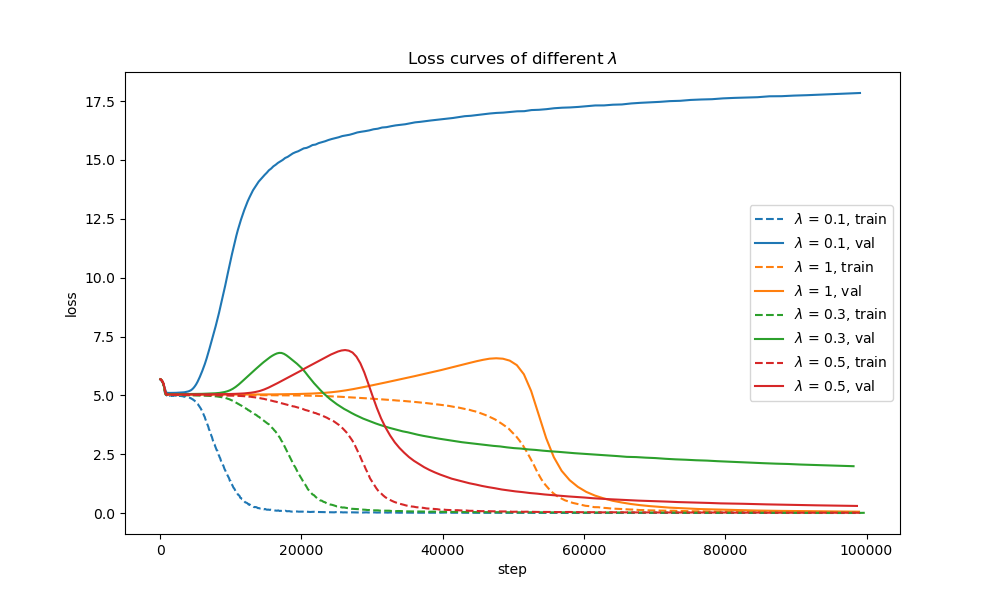
\includegraphics[width=\linewidth]{fig/loss_curves/different_Afraction_loss.png}
        \caption{Training and validation loss}
        \label{fig:different_lambda_loss}
    \end{subfigure}

    \caption{Learning curves of different target functions $f_A^*$.}
    \label{fig:acc_and_loss_different_lambda}
\end{figure}

\cref{fig:different_lambda_acc} shows that it becomes slower to overfit the training data as non-linearity $\lambda$ increases.
Perhaps surprisingly, generalization nevertheless becomes easier as $\lambda$ increases.
For $\lambda = 0.1$, the model does not generalize at all and the validation loss blows up.
For $\lambda = 0.3$ and $0.5$, some generalization happens, but the validation loss does not fully converge within $10^5$ steps.
For $\lambda = 1.0$, the model quickly generalizes after it begins to fit the training data, and the grokking phenomenon almost vanishes.

We believe this interesting result reflects the mechanism of regime transition.
For smaller $\lambda$'s, the target function $f_A^*$ behaves more like a linear function.
Hence, the model tends to first learn these linear features.
It is then trapped in the kernel regime, and have to take a long time to escape from the affine subspace $W$ and enter the rich regime;
\emph{this is how grokking happens}.
To be specific, the peaks of the loss curves in \cref{fig:different_lambda_loss} approximately corresponds to the kernel regime, and the similar shapes can also be observed in \cref{fig:loss_curve_transformer,fig:loss_curve_LSTM,fig:loss_curve_MLP}.
In contrast, For a larger $\lambda$, the function $f_A^*$ is very far from a linear map, hence forcing the model to learn other useful features.
Therefore, the model quickly moves to the rich regime and converges to the global optimal solution.
Since the transition happens immediately, grokking almost disappears in this setting.

Finally, we note that the influence of non-linearity $\lambda$ is consistent with our results in \cref{sec:subtask4}.
For $K \geq 3$, let $f^K$ and $f^{K-1}$ be the target functions of $K$-wise and $(K-1)$-wise modular addition, respectively.
No hard to see that $f^{K-1}$ is equivalent to $f^K_{\{0\}}$, which has non-linearity $\lambda = 1/p$ compared with $f^K$.
Therefore, it would be easier for $f^K$ to generalize than $f^{K-1}$.
This explains our experiment results for $K = 2, 3, 4$ in \cref{fig:grok_of_K=2_3,fig:K=4}.


\addcontentsline{toc}{section}{References}
\bibliographystyle{unsrt}
\begin{small}	
    \bibliography{ref}
\end{small}


%%%%%%%%%%%%%%%%%%%%%%%%%%%%%%%%%%%%%%%%%%%%%%%%%%%%%%%%%%%%


\appendix


\section{Appendix}


Optionally include extra information (complete proofs, additional experiments and plots) in the appendix.
This section will often be part of the supplemental material.


\end{document}
